\documentclass{article}
\usepackage[paperwidth=14.95in,paperheight=7.35in,margin=0.12in]{geometry}
\usepackage{amsmath}
\usepackage{tikz}
\usetikzlibrary{arrows.meta,positioning,calc}
\pagestyle{empty}

\begin{document}
\noindent
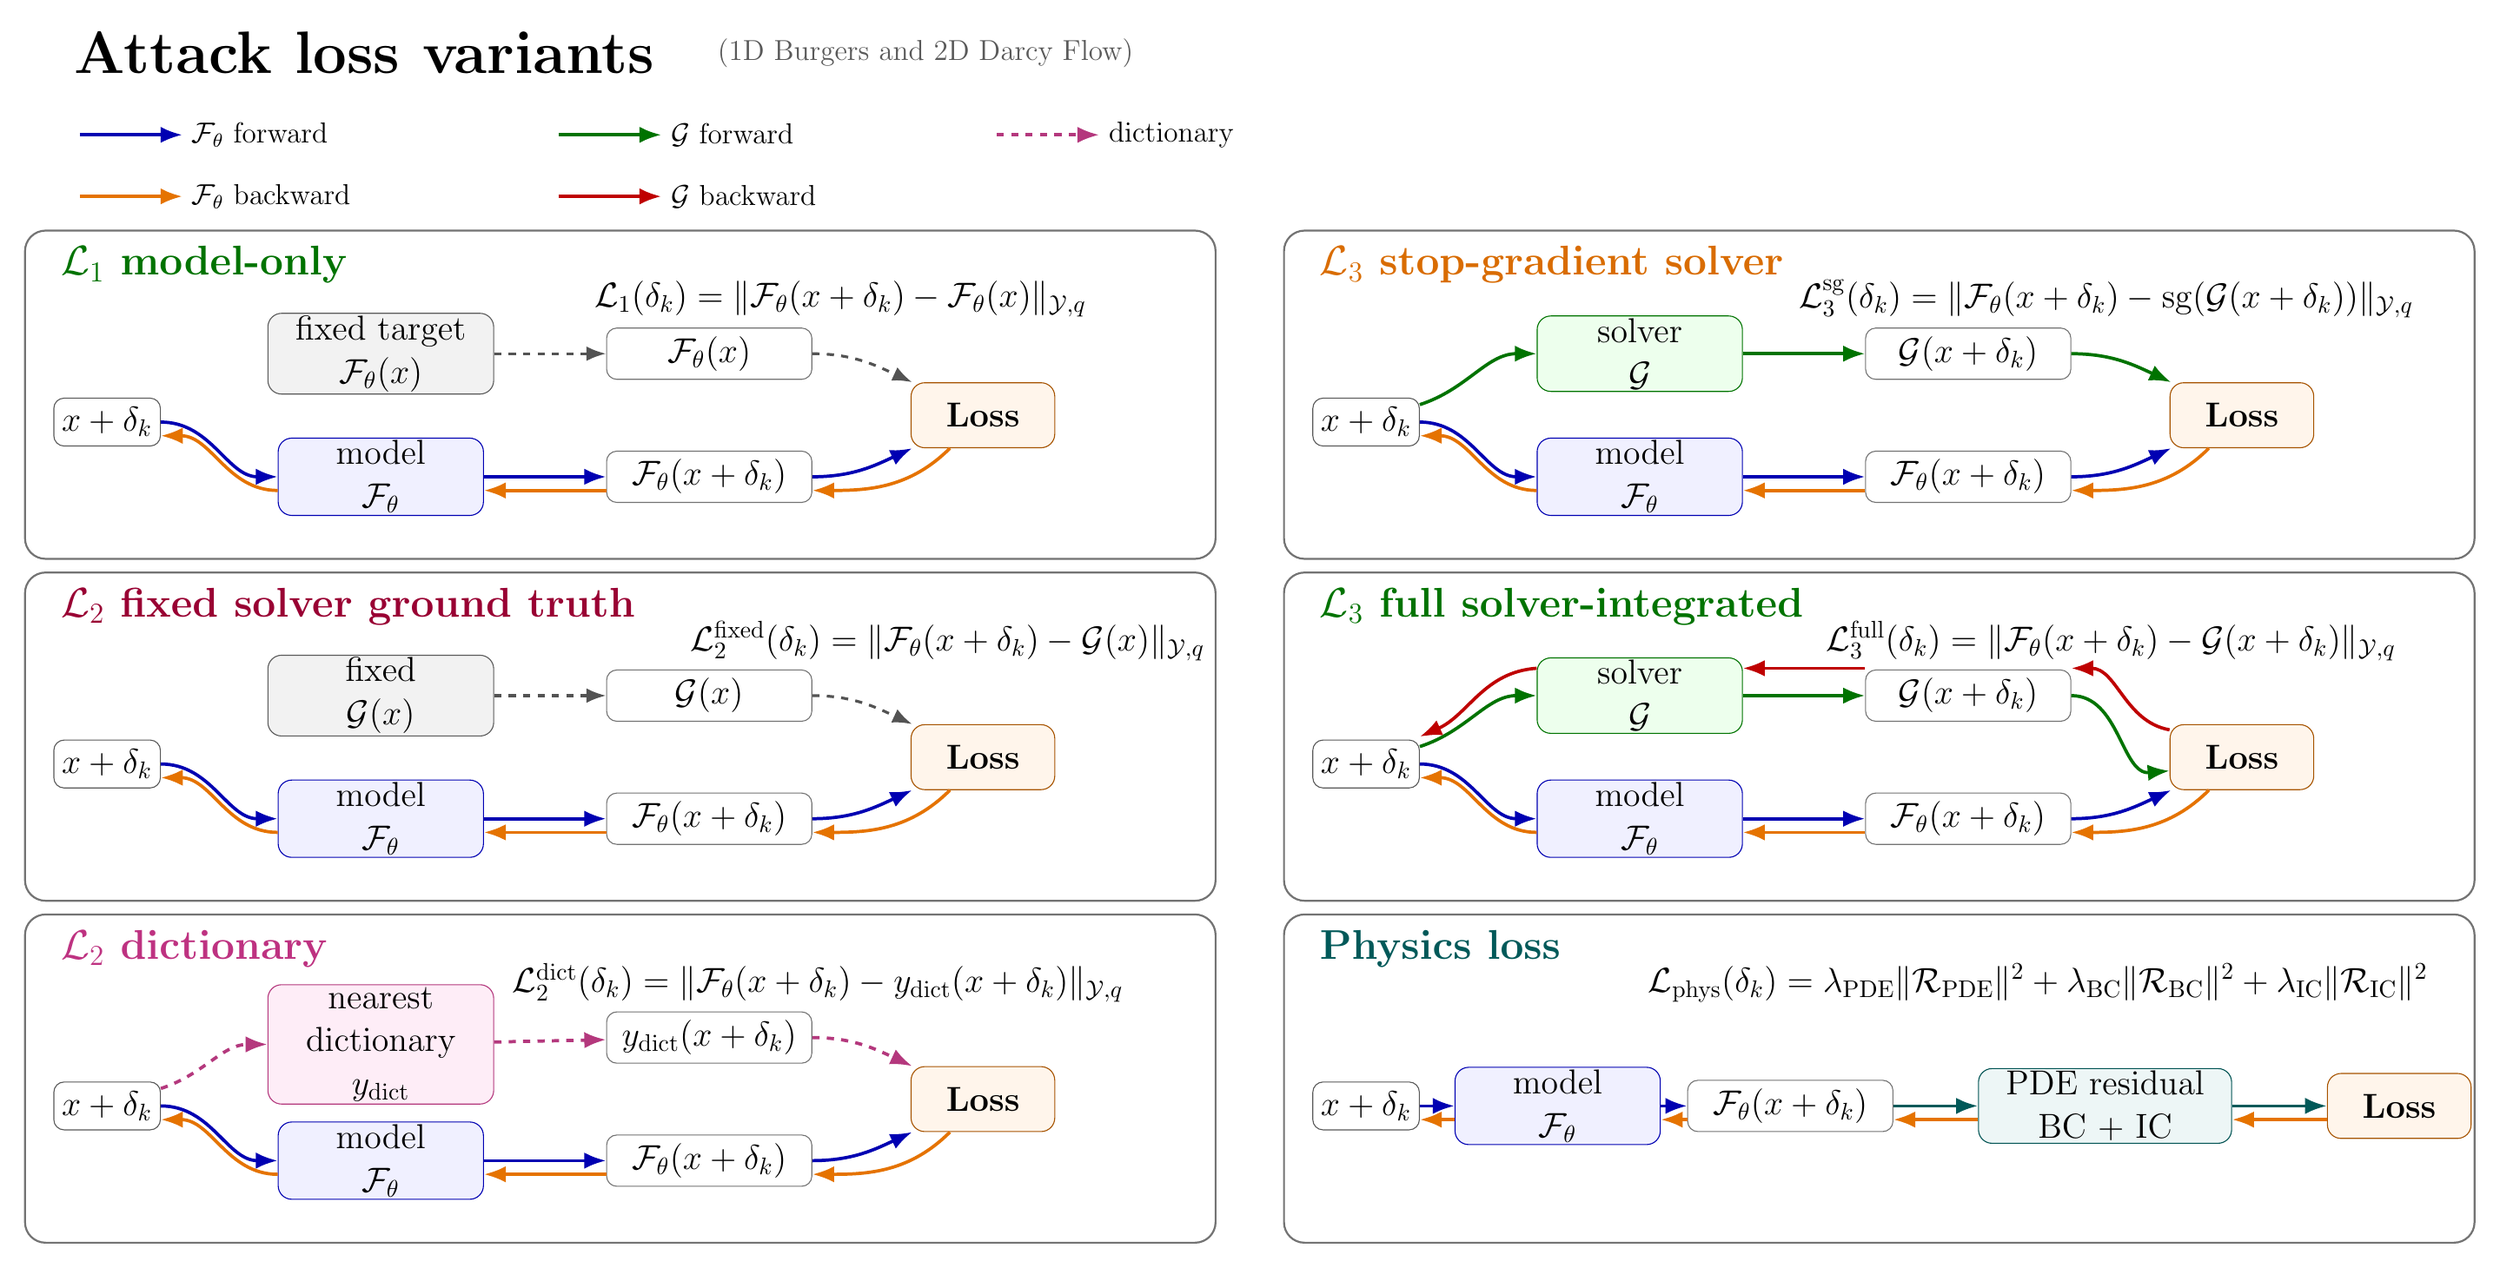
\begin{tikzpicture}[
  x=1mm,y=1mm,
  >=Latex,
  font=\sffamily,
  panel/.style={draw=black!55, rounded corners=3mm, line width=0.8pt, fill=white},
  nodebox/.style={draw=black!65, rounded corners=1.5mm, fill=white, minimum height=7mm, align=center, font=\Large, inner ysep=1pt},
  opmodel/.style={draw=blue!70!black, rounded corners=2mm, fill=blue!6, minimum width=30mm, minimum height=8.5mm, align=center, font=\Large, inner ysep=1pt},
  opsolver/.style={draw=green!45!black, rounded corners=2mm, fill=green!7, minimum width=30mm, minimum height=8.5mm, align=center, font=\Large, inner ysep=1pt},
  opdict/.style={draw=magenta!70!black, rounded corners=2mm, fill=magenta!7, minimum width=33mm, minimum height=8.5mm, align=center, font=\Large, inner ysep=1pt},
  opfixed/.style={draw=gray!70!black, rounded corners=2mm, fill=gray!10, minimum width=33mm, minimum height=8.5mm, align=center, font=\Large, inner ysep=1pt},
  opphys/.style={draw=teal!65!black, rounded corners=2mm, fill=teal!7, minimum width=37mm, minimum height=8.5mm, align=center, font=\Large, inner ysep=1pt},
  outbox/.style={draw=black!55, rounded corners=1.5mm, fill=white, minimum width=30mm, minimum height=7.5mm, align=center, font=\Large, inner ysep=1pt},
  lossbox/.style={draw=orange!65!black, rounded corners=2mm, fill=orange!8, minimum width=21mm, minimum height=9.5mm, align=center, font=\Large\bfseries, inner ysep=1pt},
  fmodel/.style={->, draw=blue!70!black, line width=1.35pt},
  fsolver/.style={->, draw=green!45!black, line width=1.35pt},
  fdict/.style={->, draw=magenta!70!black, line width=1.35pt, dashed},
  fphys/.style={->, draw=teal!70!black, line width=1.35pt},
  ffixed/.style={->, draw=gray!65!black, line width=1.15pt, dashed},
  bmodel/.style={->, draw=orange!90!black, line width=1.35pt},
  bsolver/.style={->, draw=red!75!black, line width=1.35pt},
  label/.style={font=\LARGE\bfseries, anchor=west},
  formula/.style={font=\Large, anchor=west, align=left},
  note/.style={font=\normalsize, text=black!65, anchor=west}
]

\node[font=\Huge\bfseries, anchor=west] at (6,174) {Attack loss variants};
\node[font=\large, anchor=west, text=black!65] at (100,174) {(1D Burgers and 2D Darcy Flow)};
\draw[fmodel] (8,162) -- ++(15,0) node[right, black, font=\large] {$\mathcal F_\theta$ forward};
\draw[fsolver] (78,162) -- ++(15,0) node[right, black, font=\large] {$\mathcal G$ forward};
\draw[fdict] (142,162) -- ++(15,0) node[right, black, font=\large] {dictionary};
\draw[bmodel] (8,153) -- ++(15,0) node[right, black, font=\large] {$\mathcal F_\theta$ backward};
\draw[bsolver] (78,153) -- ++(15,0) node[right, black, font=\large] {$\mathcal G$ backward};

% Panel macro geometry:
% input at x=12, model/target operator at x=52, outputs at x=100, loss at x=140.
% Two-column version: panels 1--3 on the left, panels 4--6 on the right.

% 1. L1
\begin{scope}[shift={(0,100)}]
  \draw[panel] (0,0) rectangle (174,48);
  \node[label, text=green!45!black] at (4,43) {$\mathcal L_1$ model-only};
  \node[formula] at (82,38) {$\mathcal L_1(\delta_k)=\|\mathcal F_\theta(x+\delta_k)-\mathcal F_\theta(x)\|_{\mathcal Y,q}$};

  \node[nodebox] (z) at (12,20) {$x+\delta_k$};
  \node[opfixed] (targetop) at (52,30) {fixed target\\$\mathcal F_\theta(x)$};
  \node[outbox] (targetout) at (100,30) {$\mathcal F_\theta(x)$};
  \node[opmodel] (model) at (52,12) {model\\$\mathcal F_\theta$};
  \node[outbox] (modelout) at (100,12) {$\mathcal F_\theta(x+\delta_k)$};
  \node[lossbox] (loss) at (140,21) {Loss};

  \draw[ffixed] (targetop) -- (targetout);
  \draw[ffixed] (targetout) to[out=0,in=155] (loss);
  \draw[fmodel] (z) to[out=0,in=180] (model);
  \draw[fmodel] (model) -- (modelout);
  \draw[fmodel] (modelout) to[out=0,in=205] (loss);

  \draw[bmodel] (loss) to[out=225,in=0] ([yshift=-2mm]modelout.east);
  \draw[bmodel] ([yshift=-2mm]modelout.west) -- ([yshift=-2mm]model.east);
  \draw[bmodel] ([yshift=-2mm]model.west) to[out=180,in=0] ([yshift=-2mm]z.east);
\end{scope}

% 2. L2 fixed
\begin{scope}[shift={(0,50)}]
  \draw[panel] (0,0) rectangle (174,48);
  \node[label, text=purple!80!black] at (4,43) {$\mathcal L_2$ fixed solver ground truth};
  \node[formula] at (96,38) {$\mathcal L_2^{\mathrm{fixed}}(\delta_k)=\|\mathcal F_\theta(x+\delta_k)-\mathcal G(x)\|_{\mathcal Y,q}$};

  \node[nodebox] (z) at (12,20) {$x+\delta_k$};
  \node[opfixed] (targetop) at (52,30) {fixed\\$\mathcal G(x)$};
  \node[outbox] (targetout) at (100,30) {$\mathcal G(x)$};
  \node[opmodel] (model) at (52,12) {model\\$\mathcal F_\theta$};
  \node[outbox] (modelout) at (100,12) {$\mathcal F_\theta(x+\delta_k)$};
  \node[lossbox] (loss) at (140,21) {Loss};

  \draw[ffixed] (targetop) -- (targetout);
  \draw[ffixed] (targetout) to[out=0,in=155] (loss);
  \draw[fmodel] (z) to[out=0,in=180] (model);
  \draw[fmodel] (model) -- (modelout);
  \draw[fmodel] (modelout) to[out=0,in=205] (loss);

  \draw[bmodel] (loss) to[out=225,in=0] ([yshift=-2mm]modelout.east);
  \draw[bmodel] ([yshift=-2mm]modelout.west) -- ([yshift=-2mm]model.east);
  \draw[bmodel] ([yshift=-2mm]model.west) to[out=180,in=0] ([yshift=-2mm]z.east);
\end{scope}

% 3. L2 dictionary
\begin{scope}[shift={(0,0)}]
  \draw[panel] (0,0) rectangle (174,48);
  \node[label, text=magenta!75!black] at (4,43) {$\mathcal L_2$ dictionary};
  \node[formula] at (70,38) {$\mathcal L_2^{\mathrm{dict}}(\delta_k)=\|\mathcal F_\theta(x+\delta_k)-y_{\mathrm{dict}}(x+\delta_k)\|_{\mathcal Y,q}$};

  \node[nodebox] (z) at (12,20) {$x+\delta_k$};
  \node[opdict, minimum height=12mm] (dict) at (52,29) {nearest\\dictionary\\$y_{\mathrm{dict}}$};
  \node[outbox] (targetout) at (100,30) {$y_{\mathrm{dict}}(x+\delta_k)$};
  \node[opmodel] (model) at (52,12) {model\\$\mathcal F_\theta$};
  \node[outbox] (modelout) at (100,12) {$\mathcal F_\theta(x+\delta_k)$};
  \node[lossbox] (loss) at (140,21) {Loss};

  \draw[fdict] (z) to[out=18,in=180] (dict);
  \draw[fdict] (dict) -- (targetout);
  \draw[fdict] (targetout) to[out=0,in=155] (loss);
  \draw[fmodel] (z) to[out=0,in=180] (model);
  \draw[fmodel] (model) -- (modelout);
  \draw[fmodel] (modelout) to[out=0,in=205] (loss);

  \draw[bmodel] (loss) to[out=225,in=0] ([yshift=-2mm]modelout.east);
  \draw[bmodel] ([yshift=-2mm]modelout.west) -- ([yshift=-2mm]model.east);
  \draw[bmodel] ([yshift=-2mm]model.west) to[out=180,in=0] ([yshift=-2mm]z.east);
\end{scope}

% 4. L3 stop-gradient
\begin{scope}[shift={(184,100)}]
  \draw[panel] (0,0) rectangle (174,48);
  \node[label, text=orange!85!black] at (4,43) {$\mathcal L_3$ stop-gradient solver};
  \node[formula] at (74,38) {$\mathcal L_3^{\mathrm{sg}}(\delta_k)=\|\mathcal F_\theta(x+\delta_k)-\mathrm{sg}(\mathcal G(x+\delta_k))\|_{\mathcal Y,q}$};

  \node[nodebox] (z) at (12,20) {$x+\delta_k$};
  \node[opsolver] (solver) at (52,30) {solver\\$\mathcal G$};
  \node[outbox] (solverout) at (100,30) {$\mathcal G(x+\delta_k)$};
  \node[opmodel] (model) at (52,12) {model\\$\mathcal F_\theta$};
  \node[outbox] (modelout) at (100,12) {$\mathcal F_\theta(x+\delta_k)$};
  \node[lossbox] (loss) at (140,21) {Loss};

  \draw[fsolver] (z) to[out=18,in=180] (solver);
  \draw[fsolver] (solver) -- (solverout);
  \draw[fsolver] (solverout) to[out=0,in=155] (loss);
  \draw[fmodel] (z) to[out=0,in=180] (model);
  \draw[fmodel] (model) -- (modelout);
  \draw[fmodel] (modelout) to[out=0,in=205] (loss);

  \draw[bmodel] (loss) to[out=225,in=0] ([yshift=-2mm]modelout.east);
  \draw[bmodel] ([yshift=-2mm]modelout.west) -- ([yshift=-2mm]model.east);
  \draw[bmodel] ([yshift=-2mm]model.west) to[out=180,in=0] ([yshift=-2mm]z.east);
\end{scope}

% 5. L3 full solver-integrated
\begin{scope}[shift={(184,50)}]
  \draw[panel] (0,0) rectangle (174,48);
  \node[label, text=green!45!black] at (4,43) {$\mathcal L_3$ full solver-integrated};
  \node[formula] at (78,38) {$\mathcal L_3^{\mathrm{full}}(\delta_k)=\|\mathcal F_\theta(x+\delta_k)-\mathcal G(x+\delta_k)\|_{\mathcal Y,q}$};

  \node[nodebox] (z) at (12,20) {$x+\delta_k$};
  \node[opsolver] (solver) at (52,30) {solver\\$\mathcal G$};
  \node[outbox] (solverout) at (100,30) {$\mathcal G(x+\delta_k)$};
  \node[opmodel] (model) at (52,12) {model\\$\mathcal F_\theta$};
  \node[outbox] (modelout) at (100,12) {$\mathcal F_\theta(x+\delta_k)$};
  \node[lossbox] (loss) at (140,21) {Loss};

  \draw[fsolver] (z) to[out=18,in=180] (solver);
  \draw[fsolver] (solver) -- (solverout);
  \draw[fsolver] (solverout) to[out=0,in=185] ([yshift=-2mm]loss.west);
  \draw[fmodel] (z) to[out=0,in=180] (model);
  \draw[fmodel] (model) -- (modelout);
  \draw[fmodel] (modelout) to[out=0,in=205] (loss);

  \draw[bsolver] ([yshift=4mm]loss.west) to[out=170,in=0] ([yshift=4mm]solverout.east);
  \draw[bsolver] ([yshift=4mm]solverout.west) -- ([yshift=4mm]solver.east);
  \draw[bsolver] ([yshift=4mm]solver.west) to[out=184,in=24] ([yshift=4mm]z.east);
  \draw[bmodel] (loss) to[out=225,in=0] ([yshift=-2mm]modelout.east);
  \draw[bmodel] ([yshift=-2mm]modelout.west) -- ([yshift=-2mm]model.east);
  \draw[bmodel] ([yshift=-2mm]model.west) to[out=180,in=0] ([yshift=-2mm]z.east);
\end{scope}

% 6. Physics loss
\begin{scope}[shift={(184,0)}]
  \draw[panel] (0,0) rectangle (174,48);
  \node[label, text=teal!70!black] at (4,43) {Physics loss};
  \node[formula] at (52,38) {$\mathcal L_{\mathrm{phys}}(\delta_k)=
  \lambda_{\mathrm{PDE}}\|\mathcal R_{\mathrm{PDE}}\|^2+
  \lambda_{\mathrm{BC}}\|\mathcal R_{\mathrm{BC}}\|^2+
  \lambda_{\mathrm{IC}}\|\mathcal R_{\mathrm{IC}}\|^2$};

  \node[nodebox] (z) at (12,20) {$x+\delta_k$};
  \node[opmodel] (model) at (40,20) {model\\$\mathcal F_\theta$};
  \node[outbox] (modelout) at (74,20) {$\mathcal F_\theta(x+\delta_k)$};
  \node[opphys] (residual) at (120,20) {PDE residual\\BC + IC};
  \node[lossbox] (loss) at (163,20) {Loss};

  \draw[fmodel] (z) to[out=0,in=180] (model);
  \draw[fmodel] (model) -- (modelout);
  \draw[fphys] (modelout) -- (residual);
  \draw[fphys] (residual) -- (loss);

  \draw[bmodel] ([yshift=-2mm]loss.west) -- ([yshift=-2mm]residual.east);
  \draw[bmodel] ([yshift=-2mm]residual.west) -- ([yshift=-2mm]modelout.east);
  \draw[bmodel] ([yshift=-2mm]modelout.west) -- ([yshift=-2mm]model.east);
  \draw[bmodel] ([yshift=-2mm]model.west) to[out=180,in=0] ([yshift=-2mm]z.east);
\end{scope}

\end{tikzpicture}
\end{document}
